% Copyright 2009 by Rainer Finocchiaro
% Copyright 2015 by Simon Pickartz
%
%%*****************************************
%%*                                       *
%%* RWTH Aachen University                *
%%*                                       *
%%* Institute for Automation of Complex   *
%%* Power Systems                         * 
%%*                                       *
%%* Based on the thesis template          * 
%%* of the Chair for Operating Systems    *
%%* created by Rainer Finocchiaro         *
%%*                                       *
%%*****************************************
%%
%%
%% C H A N G E L O G :
%% ~~~~~~~~~~~~~~~~~~~
%%
%% 2015/01/05 [SP]: - Initial version
%% 2015/04/23 [SP]: - First Release Candidate
%% 2015/05/21 [SP]: - Bibliography to ToC; add abstract support
%%
%%
%% [SP] Simon Pickartz
%%
%%
% Template for Master and Bachelor Theses at ACS (based on scrbook)

\documentclass[%
			   bibliography=totoc, 		% Add bibliography to toc
%				english,ngerman 		% Main language: German; second Lang: English
               ngerman,english 			% Main language: English; second Lang: German 
               ]{template/acsthesis}	

\makeindex 								% uncomment if index should be created
			   							% and uncomment '\printindex' at the bottom


\title{Analysis, Design and Implementation of a Printing Stack for the Open-Source ReactOS Operating System}
\titleDE{Analyse, Design und Implementierung eines Druckerstacks für das Open-Source ReactOS Betriebssystem}
\thesisType{bachelor} 										% 'bachelor' or 'master'
\author{Colin Finck}
\matrNr{314570}
\submissionDate{September 29, 2015}
\keywordsDE{ReactOS, Betriebssysteme, Drucken, Reverse Engineering}
\keywordsEN{ReactOS, Operating Systems, Printing, Reverse Engineering}

\addsupervisor{Dr. rer. nat. Stefan~Lankes} 			 				% Supervisor

% Whether to output the Print version (with RWTH logo) or the public version
\newboolean{outputPrintVersion}
\setboolean{outputPrintVersion}{false}

% Uncomment this to add a DRAFT watermark
%\usepackage{draftwatermark}
%\SetWatermarkText{DRAFT}
 				% Configuration (e.g., author) go into 'config.tex'
% Add further definitions and additional packages  here
\usetikzlibrary{calc, shapes, arrows, chains, decorations.text, backgrounds}

\tikzset{
	cf_base/.style={font=\sffamily\footnotesize, node distance=15mm, fill=white},
	cf_block/.style={cf_base, draw, rectangle, rounded corners, on grid, align=center},
	cf_data/.style={cf_base, draw, cylinder, aspect=0.2, on grid, shape border rotate=90]},
	cf_head/.style={font=\sffamily\bfseries\normalsize, on grid},
	cf_impl/.style={cf_base, fill=yellow!20},
	cf_label/.style={align=left, draw opacity=0, font=\sffamily\tiny},
	cf_line/.style={cf_base, draw, -latex},
	cf_skiplistitem/.style={cf_base, draw, rectangle split, rectangle split parts=#1, rectangle split empty part height=1.5ex, rectangle split empty part width=1ex, align=center}
}

% The bibliography
\usepackage[backend=bibtex, style=numeric]{biblatex}
\addbibresource{bibliography}

% package for glossary
\usepackage[nopostdot, nonumberlist, nogroupskip, toc]{glossaries}
\usepackage{glossary-mcols}

% package for algorithms in pseudocode
\usepackage{algorithm}
\usepackage{algpseudocode}
\usepackage{amssymb}

% package for plots
\usepackage{pgfplots}

% support for landscape figures
\usepackage{rotating}
\usepackage{pdflscape}

% package for listings
\usepackage{listings}

\definecolor{bluekeywords}{rgb}{0, 0, 1}
\definecolor{greencomments}{rgb}{0, 0.5, 0}
\definecolor{redstrings}{rgb}{0.64, 0.08, 0.08}

\lstset{
	language=C++,
	captionpos=b,
	frame=lines,
	showspaces=false,
	showtabs=false,
	breaklines=true,
	showstringspaces=false,
	breakatwhitespace=true,
	commentstyle=\color{greencomments},
	keywordstyle=\color{bluekeywords},
	morekeywords={__inline},
	stringstyle=\color{redstrings},
	basicstyle=\ttfamily\small,
}

% Hyphenation settings for some words
\selectlanguage{ngerman}
\hyphenation{ReactOS}
\selectlanguage{english}
\hyphenation{ReactOS}

% Prevent single lines to be printed on the next page
\clubpenalty = 10000
\widowpenalty = 10000 
\displaywidowpenalty = 10000
				% Additional definitions and packages
% This is the glossary file for my thesis
\newglossarystyle{myglossarystyle}{               % new glossary style
   \setglossarystyle{long}                           % based on style long
   \renewenvironment{theglossary}
   {\begin{longtable}
      {@{}p{0.25\textwidth} p{0.7\textwidth}}}   % adjust width of columns
   {\end{longtable}}
   \renewcommand*{\glsgroupskip}{}               % no grouping
}
 
\setglossarystyle{myglossarystyle}
 
\makeglossaries

\newacronym{API}{API}{Application Programming Interface}
\newacronym{AVL}{AVL}{Adelson-Velski Landis}
\newacronym{BIOS}{BIOS}{Basic Input/Output System}
\newacronym{CUPS}{CUPS}{Common UNIX Printing System}
\newacronym[longplural={Dynamic Link Libraries}]{DLL}{DLL}{Dynamic Link Library}
\newacronym{EMF}{EMF}{Enhanced Metafile}
\newacronym{GDI}{GDI}{Graphics Device Interface}
\newacronym{HTTP}{HTTP}{Hyper-Text Transfer Protocol}
\newacronym{IDL}{IDL}{Interface Definition Language}
\newacronym{IPP}{IPP}{Internet Printing Protocol}
\newacronym{KD}{KD}{Kernel Debugging}
\newacronym{LCG}{LCG}{Linear Congruential Generator}
\newacronym{LPD}{LPD}{Line Printer Daemon}
\newacronym{MIME}{MIME}{Multipurpose Internet Mail Extensions}
\newacronym{PDB}{PDB}{Program Database}
\newacronym{PDF}{PDF}{Portable Document Format}
\newacronym{PPA}{PPA}{Printing Performance Architecture}
\newacronym{PE}{PE}{Portable Executable}
\newacronym{RCE}{RCE}{Reverse Code Engineering}
\newacronym{RMI}{RMI}{Remote Method Invocation}
\newacronym{RPC}{RPC}{Remote Procedure Call}
\newacronym{SMB}{SMB}{Server Message Block}
\newacronym{STL}{STL}{Standard Template Library}
\newacronym{USB}{USB}{Universal Serial Bus}
\newacronym{XML}{XML}{Extensible Markup Language}
 % load glossary file

\begin{document}
\printglossary[type=\acronymtype, title=Abbreviations]
\listoffigures
%\listoftables	
%\lstlistoflistings
\chapter{Introduction}
\href{https://reactos.org}{ReactOS} is a modern desktop operating system entirely available under Open-Source licenses.
The Project is unique in the way that it aims for compatibility with all existing applications and drivers developed for Microsoft Windows.
This exclusive feature among free operating systems can make ReactOS an appealing alternative to the currently dominant desktop operating system.
By being distributed under Open-Source licenses, ReactOS can offer customizations and trustworthiness not possible with traditional closed-source systems.

Printing has become an essential feature of graphical desktop operating systems in the 1980 years.
The introduction of affordable Inkjet and Laser Printers around the same time have turned Personal Computers into Desktop Publishing machines able to produce high-quality documents \cite{leurs2013postscript}.
Since then, computers have mostly replaced traditional typewriters and typesetter systems.

Today, Printing is a self-evident ability of Personal Computers.
A desktop operating system is expected to detect and install connected Printers automatically as well as to provide intuitive options to manage and use them.
One of the common tasks of server operating systems is making a Printer available to multiple users over the network.
More recently, also smartphone and tablet operating systems have added support for Printing \cite{aosp2015kitkat}.
However, the ReactOS Operating System has not offered any support for Printing yet.

Operating system support for Printing also plays an important role in document exchange.
Creating a document in Adobe's popular \gls{PDF} is usually realized through a virtual Printer.
Such a Printer can be used as a destination from any text processing application just like a real Printer.


\section{Thesis Work}
This thesis presents an initial design and implementation of a Printing Stack for the ReactOS Operating System.

While several Open-Source Printing Systems already exist, none of them provides compatibility to the wide range of available Windows Printer Drivers.
On the other hand, hardware vendors often provide the most feature-rich drivers only for the Windows platform.
Therefore, the work does not build upon an existing Open-Source Printing System, but new components are developed from scratch.

In order to achieve ReactOS' goal of full compatibility to Microsoft Windows applications and drivers, the Windows Printing interfaces are analyzed in-depth.
Additionally, existing code of the ReactOS Operating System is examined to determine the extent of the required implementation work.
In a next step, a set of fundamental components is developed, which form an initial Printing Stack.
This system is able to transmit prepared RAW data in a Printer Control Language to a locally connected Printer.
However, the entire architecture is designed for a further extension by other datatypes at a later stage.

Evaluation of the written code occurs with the help of specific individual unit tests covering the implemented features.

Although Microsoft provides a publicly available documentation about their Printing implementation, it does not cover specific internals.
Therefore, a special emphasis has been put on commenting and documenting the resulting code to serve as a future reference.


\section{Special Thanks}
I would like to thank Univ. Prof. Dr.-Ing. Antonello~Monti and Dr. rer. nat. Stefan~Lankes for offering me the unique opportunity to make ReactOS part of my Bachelor thesis.
Special thanks also go to all members of the ReactOS Project who are maintaining this great Open-Source Project for several years.

\bigskip

\textit{\\
Colin Finck\\
Aachen, September 2015
}
% These abbreviations are used in figure labels and all figures are listed in the "List of Figures" some pages before.
% Reset them, so that they are expanded once in the text.
\glsreset{API}
\glsreset{PDB}
\glsreset{RPC}

\chapter{Basics}
This chapter introduces several Open-Source software projects relevant to the thesis implementation work.
It is followed by an explanation of the backgrounds and technical terms regarding Printing support in operating systems.
Finally, some utilities are presented, which have been widely used for the development of the Printing Stack.


\section{The ReactOS Project}
The ReactOS Project goes back to a project called \emph{FreeWin95} in 1996 by various software developers to create an Open-Source reimplementation of Microsoft Windows 95.
With no visible progress by the end of 1997, the project was restarted in 1998 as \emph{ReactOS} and shifted its goals towards providing an operating system compatible with the Microsoft Windows NT series under the GNU General Public License \cite{reactos1998news}.
The name was chosen to express the dissatisfaction with the Microsoft operating system monopoly and provide a \emph{reaction} to it \cite{sixtus2004reactos}.

Today, ReactOS strives for compatibility with Windows Server 2003 (also known as Windows NT 5.2) at the kernel level while applications can also make use of some functions found in more recent Windows releases \cite{guo2009newsletter54}.
Several popular Windows applications such as Adobe Photoshop or Microsoft Office are running natively under ReactOS.
This also applies to several drivers for hardware components such as graphics adapters, network cards, or sound cards.

By providing this level of compatibility with a very popular operating system, ReactOS aims to become a free and Open-Source alternative to it.
As a lightweight operating system, ReactOS can be a solution to keep older computers usable.
Finally, the Open-Source nature of ReactOS allows for customizations not possible with Microsoft Windows.
It also reduces licensing costs and ensures confidentiality in sensitive environments.


\section{The WINE Project}
The Open-Source WINE Project was founded in 1993 with the goal of running Windows applications under Linux.
In contrast to typical emulator software, WINE does not simulate a full x86 processor to run an operating system on it, but instead provides a loader for binaries in the Windows \gls{PE} format along with a set of reimplemented Windows libraries \cite{gardner1998winefaq}.
This allows applications to deliver a higher performance under WINE than under x86 emulators, but this performance benefit is getting lower with advancements in x86 virtualization technology.

In contrast to ReactOS, WINE does not provide any support for Windows device drivers.
The project also does not target a specific Windows version, but allows users to choose a particular Windows version WINE shall mimic.
Due to similar licenses, code of fundamental Windows libraries is frequently exchanged between the ReactOS and the WINE Project.


\section{Printing Support In Operating Systems}
Operating system support for Printing is as old as the Personal Computer itself, with support for then standard Dot-Matrix Parallel Port Printers being implemented into the original IBM Personal Computer 5150 \gls{BIOS} of 1981 \cite{brooks2015pcdos, powell2010lprng}.
As neither a concept of Printer Drivers nor a common Printer Control Language existed at that time, user programs were only able to output basic unformatted text by default.
Higher sophisticated printing of different fonts or graphics required software developers to implement support for each Printer Control Language into their applications.
This first changed with the introduction of the Apple LaserWriter Printer in 1985, which standardized Adobe PostScript as a vendor-independent Printer Control Language \cite{leurs2013postscript}.
Around the same time Windows 1.0 debuted, featuring a first Printing Stack consisting of a Print Spooler along with a set of Printer Drivers for converting \gls{GDI} output into different Printer Control Languages \cite{kolacki1987windows}.
Instead of talking directly to the Printer, applications now just needed to call \gls{GDI} functions for printing out a document. Usually, these are the same functions already used for displaying graphics and text on the screen.
The Spooler is responsible for enabling non-blocking access to a single shared Printer by multiple applications.

With Windows, Mac OS X, and Linux evolving into the three popular operating systems these days, two Printing Stacks remain.
These are described in the following sections.

\subsection{Microsoft Windows Printing Stack}
\label{sec:WindowsPrinting}
The Printing Stack of the Microsoft Windows Operating System is unique in the way that some higher level components maintain compatibility with all previous Windows versions. At the same time, lower level parts follow the latest principles of modern operating systems.
A schema of the Printing Process under Windows 2000 and later is given in Figures~\ref{fig:WindowsSpooling} and \ref{fig:WindowsPrinting}.
All components involved are explained in the following.
Yellow marked nodes denote components, for which compatible replacements are implemented within this thesis.

\begin{figure}[h]
	\centering
	
	\begin{tikzpicture}
		\node [cf_block, cf_impl] (App) {Application};
		\node [cf_block, below left = 20mm of App] (gdi32) {GDI\\gdi32.dll};
		\node [cf_block, cf_impl, below = 30mm of App] (winspool) {Spooler API\\winspool.drv};
		\node [cf_block, cf_impl, below = 20mm of winspool] (spoolsv) {Spooler Server\\spoolsv.exe};
		\node [cf_block, cf_impl, below = of spoolsv] (spoolss) {Spooler Router\\spoolss.dll};
		\node [cf_block, cf_impl, below left = 20mm and 32mm of spoolss] (localspl) {Local Spooler\\localspl.dll};
		\node [cf_block, below = 20mm of spoolss] (inetpp) {Internet Print Provider\\inetpp.dll};
		\node [cf_block, below right = 20mm and 40mm of spoolss] (win32spl) {LanMan Print Services\\win32spl.dll};
		\node [cf_block, right = 80mm of spoolsv] (extern_spoolsv) {Spooler Server\\on another computer};
		\node [cf_data, cf_impl, below = 20mm of localspl] (spoolfile) {Spool File};
		\node [cf_block, below = 20mm of inetpp] (ippprinter) {IPP-capable Printer};
		
		\path [cf_line, dotted] (App) -- (gdi32);
		\path [cf_line, dotted] (App) -- (winspool);
		\path [cf_line] (gdi32) -- (winspool);
		\path [cf_line] (winspool) -- (spoolsv);
		\path [cf_label] (winspool) edge node [right] {RPC Calls over\\ncalrpc protocol} (spoolsv);
		\path [cf_line] (spoolsv) -- (spoolss);
		\path [cf_line, dotted] (spoolss) -- (localspl);
		\path [cf_line, dotted] (spoolss) -- (inetpp);
		\path [cf_line, dotted] (spoolss) -- (win32spl);
		\path [cf_line] (localspl) -- (spoolfile);
		\path [cf_line] (inetpp) -- (ippprinter);
		
		\coordinate [left = 3mm of extern_spoolsv] (extern_spoolsv_anchor);
		\path [draw] (win32spl) -- (win32spl |- ippprinter.north);
		\path [draw] (win32spl |- ippprinter.north) -- (ippprinter.north -| extern_spoolsv_anchor);
		\path [draw] (ippprinter.north -| extern_spoolsv_anchor) -- (extern_spoolsv_anchor);
		\path [cf_label] (ippprinter.north -| extern_spoolsv_anchor) edge node [right] {RPC Calls over\\ncacn\_np protocol} (extern_spoolsv_anchor);
		\path [cf_line] (extern_spoolsv_anchor) -- (extern_spoolsv.west);
	\end{tikzpicture}
	
	\caption{Spooling a Print Job into a file as implemented in current Microsoft Windows Operating Systems}
	\label{fig:WindowsSpooling}
\end{figure}

User-Mode Windows applications interact with the operating system by calling documented \gls{API} functions from operating system \gls{DLL} files.
To print out a document, an application usually begins by composing the document out of graphics and text using \gls{GDI} functions (implemented in \emph{gdi32.dll}).
Afterwards, \gls{GDI} serializes the drawing commands into the \gls{EMF} format and uses Spooler \gls{API} functions to set up a new Print Job.
The generated \gls{EMF} data is then passed to the Print Job.
If the application does not need to compose the document, but already has prepared data in a format supported by the Print Processor, it can skip the route through \gls{GDI} and call the Spooler \gls{API} functions directly \cite{yuan2001windows}.

For historical reasons, the Spooler \gls{API} is implemented in a file called \emph{winspool.drv}.
Despite its different extension, this file has the same structure as other operating system \gls{DLL} files.
An individual instance of \emph{winspool.drv} is loaded with every application that uses functions of the Windows Printing Stack.
Its \gls{API} can be categorized as follows:

\begin{itemize}
	\item Opening handles to Ports, Print Monitors, Print Servers, and Printers (all through \texttt{OpenPrinter} \cite{msdn2015openprinter})
	\item Performing further operations on these opened objects (e.g. preparing a new document with \texttt{StartDocPrinter} or retrieving information with \texttt{GetPrinter})
	\item Adding, deleting, and enumerating available Forms, Ports, Print Monitors, Print Processors, Printers, Printer Configuration Data, Printer Connections, and Printer Drivers as well as their properties (\texttt{Add*}, \texttt{Delete*}, and \texttt{Enum*} group of functions)
	\item Receiving notifications about status changes inside the Printing Stack \\ (\texttt{*PrinterChangeNotification} group of functions)
	\item Providing User Interfaces to let the user configure Printer and Print Job settings
\end{itemize}

As every application loads its own instance of \emph{winspool.drv}, the operating system needs to provide a single service, which is loaded only once and centrally manages Printer utilization.
This instance is the Spooler Server, which is implemented as a Windows Service in the module \emph{spoolsv.exe}.
Communication between \emph{winspool.drv} and \emph{spoolsv.exe} happens through \glspl{RPC}.
\gls{RPC} is a popular concept for enabling a process to call a function in another process, even on another computer, without writing any network-specific code.
Almost every \emph{winspool.drv} function performs an \gls{RPC} call to the matching counterpart function in the Spooler Server.
\gls{RPC} calls are further discussed in Section~\ref{sec:rpc}.

Accepting \gls{RPC} calls of all users requires the Spooler Server to be a high-privileged process.
This bears some security risks as a possibly vulnerable \gls{RPC} call could be used to let a low-privileged client run code in the security context of the high-privileged Spooler Server.
To mitigate this possible attack, the Spooler Server employs the concept of \emph{Impersonation}.
The Impersonation feature of Windows allows a thread to temporarily drop its high privileges by switching to the security context of another user \cite{technet2015impersonation}.

In the case of the Spooler Server, every \gls{RPC} call is implemented as follows:
First of all, the Spooler Server impersonates the calling client.
Afterwards, a matching function in the Spooler Router is called (implemented in \emph{spoolss.dll}).
The Spooler Router offers such a counterpart to each \gls{RPC} call.
Finally, the security context of the Spooler Server is restored and the \gls{RPC} call returns.
This ensures a clean separation between code running in the high-privileged Spooler Server security context and code running in the low-privileged user context.
The entire process is exemplified for a \texttt{WritePrinter} call in Figure~\ref{fig:WritePrinterProcessing}.
The full listing for the implemented ReactOS \gls{RPC} server function can be found in Appendix~\ref{sec:RpcWritePrinter}.

\begin{figure}[h]
	\centering
	
	\begin{tikzpicture}
		\node [cf_head, minimum width = 68mm] (UserContext) {Low-privileged User Context};
		\node [cf_head, minimum width = 68mm, right = 73mm of UserContext] (SystemContext) {High-privileged System Context};
	
		\node [cf_block, below = of UserContext] (App) {Application calls \texttt{WritePrinter}\\in \emph{winspool.drv}};
		\node [cf_block, below = 22mm of App] (RpcWritePrinter) {\emph{winspool.drv} calls \texttt{\_RpcWritePrinter}\\to perform an RPC call to\\the Spooler Server};
		\node [cf_block, below = 60mm of SystemContext] (RpcImpersonateClient) {Spooler Server calls\\\texttt{RpcImpersonateClient}\\to impersonate the caller};
		\node [cf_block, below = 43mm of RpcWritePrinter] (WritePrinter) {Spooler Server calls matching\\\texttt{WritePrinter} in Spooler Router};
		\node [below = 5mm of WritePrinter] (Additional) {...};
		\node [cf_block, below = 12mm of Additional] (RpcRevertToSelf) {Spooler Server calls \texttt{RpcRevertToSelf}\\to switch back to its own security context};
		\node [cf_block, below = 63mm of RpcImpersonateClient] (Return) {Spooler Server returns the\\error code of its performed\\\texttt{WritePrinter} call};
		
		\path [cf_line] (App) -- (RpcWritePrinter);
		
		\coordinate [below = 3mm of RpcWritePrinter] (RpcWritePrinter_anchor);
		\path [draw] (RpcWritePrinter) -- (RpcWritePrinter_anchor);
		\path [draw] (RpcWritePrinter_anchor) -- (RpcWritePrinter_anchor -| RpcImpersonateClient);
		\path [cf_line] (RpcWritePrinter_anchor -| RpcImpersonateClient) -- (RpcImpersonateClient);
		
		\coordinate [below = 3mm of RpcImpersonateClient] (RpcImpersonateClient_anchor);
		\path [draw] (RpcImpersonateClient) -- (RpcImpersonateClient_anchor);
		\path [draw] (RpcImpersonateClient_anchor) -- (RpcImpersonateClient_anchor -| WritePrinter);
		\path [cf_line] (RpcImpersonateClient_anchor -| WritePrinter) -- (WritePrinter);
		
		\path [draw] (WritePrinter) -- (Additional);
		\path [cf_line] (Additional) -- (RpcRevertToSelf);
		
		\coordinate [below = 3mm of RpcRevertToSelf] (RpcRevertToSelf_anchor);
		\path [draw] (RpcRevertToSelf) -- (RpcRevertToSelf_anchor);
		\path [draw] (RpcRevertToSelf_anchor) -- (RpcRevertToSelf_anchor -| Return);
		\path [cf_line] (RpcRevertToSelf_anchor -| Return) -- (Return);
		
		\coordinate [below = 2mm of Return] (Return_anchor);
		
		\begin{pgfonlayer}{background}
			\fill [fill=green!20] (UserContext.north west) rectangle (UserContext.east |- Return_anchor);
			\fill [fill=red!20] (SystemContext.north west) rectangle (SystemContext.east |- Return_anchor);
		\end{pgfonlayer}
	\end{tikzpicture}
	
	\caption{Using Impersonation to switch between security contexts while processing an \texttt{WritePrinter} call}
	\label{fig:WritePrinterProcessing}
\end{figure}

The Spooler Router derives the name from its principal task, namely routing an incoming function call to one or more Print Providers.
These Print Providers also offer a counterpart to each function implemented in the Spooler Router.
Due to the nature of the functions, there are basically three ways how a Spooler Router function is implemented:

\begin{itemize}
	\item Subsequently route a function call to every available Print Provider until one of them indicates success.
	      This is done for e.g. the \texttt{OpenPrinter} function to determine the Print Provider that can handle the respective Printer.
	\item Directly route the function call to the Print Provider, for which a previous \texttt{OpenPrinter} call succeeded.
	      This is done for all functions accepting a handle returned by \texttt{OpenPrinter}.
	\item Route the function call to all available Print Providers and collect the returned information.
	      This is done for e.g. \texttt{EnumPrinters} to retrieve information about all available Printers.
\end{itemize}

Windows ships with these Print Providers by default:

\begin{itemize}
	\item The Local Spooler (implemented in \emph{localspl.dll}) handles Printers locally connected to the computer.
	\item The Internet Print Provider (implemented in \emph{inetpp.dll}) forwards calls to Remote Printers using the \gls{IPP}.
	\item The LanMan Print Services (implemented in \emph{win32spl.dll}) are used when accessing Remote Printers shared by another Windows computer.
\end{itemize}

Another Print Provider (\emph{nwprovau.dll}) for accessing Printers on Novell NetWare servers used to be available, but became largely irrelevant due to the demise of the NetWare Operating System.
It has finally been removed in Windows Vista.
The extensible architecture enables third-party vendors to ship additional Print Providers for supporting other protocols.

In the following, we only take a look at the Local Spooler.
The Local Spooler finally does the real work of managing the Print Queues for all locally connected Printers instead of passing on the received function call to another module.
Synchronous communication between computers and Printers can be a major bottleneck.
Therefore, the Local Spooler first writes the received data to print into a so called Spool File and then starts a thread to transmit that Spool File to the Printer.
This enables the users to continue their work in the application while the Local Spooler transmits the Spool File to the Printer in the background.
Without this two-stage process, the application would be blocked until the last page of the entire Print Job has finished printing.

\begin{figure}[h]
	\centering
	
	\begin{tikzpicture}
		\node [cf_data, cf_impl] (spoolfile) {Spool File};
		\node [cf_block, cf_impl, right = 30mm of spoolfile] (winprint) {Print Processor\\winprint.dll};
		\node [cf_block, right = 50mm of winprint] (printerdll) {Printer Driver\\Graphics DLL};
		\node [cf_block, below right = 18mm of printerdll] (gdi32) {GDI\\gdi32.dll};
		\node [cf_block, cf_impl, below = 20mm of winprint] (spoolss) {Spooler Router\\spoolss.dll};
		\node [cf_block, cf_impl, below = of spoolss] (localspl) {Local Spooler\\localspl.dll};
		\node [cf_block, below = 20mm of localspl] (pjlmon) {Language Monitor\\pjlmon.dll};
		\node [cf_block, cf_impl, below left = 28mm of pjlmon] (localmon) {Local Port Monitor\\localmon.dll};
		\node [cf_block, below right = 28mm of pjlmon] (usbmon) {USB Port Monitor\\usbmon.dll};
		\node [cf_block, below = 35mm of pjlmon] (kernel32) {User-Mode Kernel API for accessing a port\\kernel32.dll};
		\node [cf_block, below = of kernel32] (printer) {Printer};
		
		\path [cf_line] (spoolfile.east) -- (winprint.west);
		\path [cf_line, dotted] (winprint.east) -- (printerdll);
		\path [cf_label] (winprint.east) edge node [above] {For EMF datatype} (printerdll);
		\path [cf_line] (printerdll) -- (gdi32);
		\path [cf_line] (gdi32.100) -- (printerdll.-30);
		\path [draw] (printerdll) -- (printerdll |- spoolss);
		\path [cf_line] (printerdll |- spoolss) -- (spoolss);
		\path [cf_label] (printerdll |- spoolss) edge node [above] {Converted to RAW datatype} (spoolss);
		\path [cf_line, dotted] (winprint) -- (spoolss);
		\path [cf_label] (winprint) edge node [right] {For RAW datatype} (spoolss);
		\path [cf_line] (spoolss) -- (localspl);
		\path [cf_line, dotted] (localspl) -- (pjlmon);
		
		\coordinate [below = 3mm of pjlmon] (pjlmon_anchor_half);
		\coordinate [below = 6mm of pjlmon] (pjlmon_anchor);
		\path [cf_line] (pjlmon) -- (pjlmon_anchor);
		\path [cf_line, dotted] (pjlmon_anchor) -- (localmon);
		\path [cf_line, dotted] (pjlmon_anchor) -- (usbmon);
	
		\coordinate [below right = 9mm of localspl] (localspl_anchor);
		\path [draw, dotted] (localspl.-40) -- (localspl.-40 |- localspl_anchor);
		\path [draw, dotted] (localspl.-40 |- localspl_anchor) -- (localspl_anchor);
		\path [draw, dotted] (localspl_anchor) -- (localspl_anchor |- pjlmon_anchor_half);
		\path [cf_line, dotted] (localspl_anchor |- pjlmon_anchor_half) -- (pjlmon_anchor_half);
		
		\path [cf_line] (localmon) -- (kernel32.north -| localmon);
		\path [cf_line] (usbmon) -- (kernel32.north -| usbmon);
		\path [cf_line] (kernel32) -- (printer);
	\end{tikzpicture}
	
	\caption{Printing from a Spool File as implemented in current Microsoft Windows Operating Systems}
	\label{fig:WindowsPrinting}
\end{figure}

The started thread now loads the Print Processor (implemented in \emph{winprint.dll} since Windows Vista, previously part of \emph{localspl.dll}), which is responsible for reading the print data from the Spool File and applying Print Job specific settings.
These include settings like Multiple Copies, Collation, Reverse Printing, Duplex Printing or N-up Printing.
Available options in this regard highly depend on the datatype of the print data.
A Printer vendor can provide its own Print Processor to support additional options instead of using the Windows default one.

If the datatype is RAW, the print data is assumed to be of a Printer Control Language and the Print Processor simply passes it on without any further processing.
For the \gls{EMF} datatype, Print Job specific settings are applied first before the print data is converted into Printer Control Language.
The conversion is performed using a Printer Graphics \gls{DLL} supplied by the Printer vendor, which heavily uses functions from \gls{GDI} to convert the \gls{EMF} data.
The Printer Graphics \gls{DLL} is also called the actual Printer Driver, because it is the only component specific to the Printer in this process.

In a next step, Spooler Router functions are used to transmit the print data in a Printer Control Language to a Print Monitor.
Two types of Print Monitors exist: Language Monitors and Port Monitors.
A Language Monitor is written for a specific Printer Job Language to communicate bidirectionally with the Printer.
This communication enables the Monitor to receive detailed Printer status information or add control codes to the print data before passing it to the Port Monitor.
Control codes can be used to set a wide range of options.
One example is switching between multiple Printer Control Languages supported by the Printer.

If the Printer does not require such control codes, the Language Monitor can be skipped and the print data directly flows to the Port Monitor.
By default, Windows ships with a Language Monitor that implements the HP PJL Printer Job Language \cite{msdn2015langmonitors}.

A Port Monitor is responsible for managing unidirectional data output to a physical computer port.
Depending on the type of port, this can range from simply opening the port through a kernel function (like Parallel Ports) to performing a complex wireless detection sequence (for Infrared Printers).
The following Port Monitors are shipped with Windows:

\begin{itemize}
	\item The Local Port Monitor (implemented in \emph{localmon.dll} until Windows NT 4.0, part of \emph{localspl.dll} since Windows 2000) manages Parallel, Serial, and Infrared Ports as well as redirecting the printing output into a file.
	\item The USB Port Monitor (implemented in \emph{usbmon.sys}) manages Printers connected to a \gls{USB} port.
\end{itemize}

This architecture again provides support for additional Print Monitors.
Such extensibility is heavily used by third-party companies.
For example, Adobe has implemented a \gls{PDF} Port Monitor for a virtual \gls{PDF} Printer that converts the print data into a \gls{PDF} file \cite{adobe2015printerproperties}.


\subsection{Common UNIX Printing System (CUPS)}
The \gls{CUPS} was developed and released by Michael Sweet in 1999 to address the lack of a standard printing interface in UNIX-based operating systems (such as Linux) at that time \cite{sweet1999cups}.
Previously, there were two competing systems, namely the System V Printing System (lp) and the Berkeley Printing System (lpr), which were incompatible to each other and only supported text and PostScript printing.
Printing other formats required third-party tools to account for the vast majority of available Printers.

\gls{CUPS} has quickly emerged as the de-facto standard Printing Stack under Linux, with User Interfaces being available for the two major desktops KDE and GNOME \cite{pfeifle2001kdeprint} \cite{burton2003gnome}.
\gls{CUPS} has also been adopted by Apple in 2002 to serve as the Printing System for Mac OS X 10.2 and later versions \cite{esp2002applecups}.

The architecture of \gls{CUPS} is depicted in Figure~\ref{fig:CUPSArchitecture}.

\begin{figure}[h]
	\centering
	
	\begin{tikzpicture}
		\node [cf_block] (app) {Application};
		\node [cf_block, below left = 15mm and 20mm of app] (cups-lpd) {cups-lpd Daemon};
		\node [cf_block, below = 30mm of app] (cupsapi) {CUPS\\API};
		\node [cf_block, below = of cupsapi] (cupsd) {CUPS Daemon};
		\node [cf_block, below = of cupsd] (prefilter) {Prefilter};
		\node [cf_block, below left = 15mm of prefilter] (pstops) {pstops};
		\node [cf_block, below left = 20mm and 12mm of pstops] (foomatic-rip) {foomatic-rip};
		\node [cf_block, below right = 12mm and 18mm of pstops] (pstoraster) {pstoraster};
		\node [cf_block, below = of pstoraster] (printerfilter) {Printer-specific\\filter};
		\node [cf_block, below = 50mm of prefilter] (backend) {CUPS Backend};
		\node [cf_block, below = of backend] (printer) {Printer};
		
		\path [cf_line, dotted] (app) -- (cups-lpd);
		\path [cf_label] (app) edge node [left] {LPD protocol} (cups-lpd);
		\path [cf_line, dotted] (app.-20) -- (app.-20 |- cupsd.north);
		\path [cf_label] (app.-20) edge node [right] {IPP protocol} (app.-20 |- cupsd.north);
		\path [cf_line, dotted] (app) -- (cupsapi);
		\path [cf_line] (cups-lpd) -- (cupsapi);
		\path [cf_line] (cupsapi) -- (cupsd);
		\path [cf_label] (cupsapi) edge node [left] {IPP protocol} (cupsd);
		\path [cf_line, dotted] (cupsd) -- (prefilter);
		\path [cf_line, dotted] (pstops |- cupsd.south) -- (pstops);
		\path [cf_line, dotted] (prefilter) -- (pstops);
		\path [cf_line, dotted] (pstops) -- (foomatic-rip);
		\path [cf_line, dotted] (pstops.-50) -- (backend.north -| pstops.-50);
		\path [cf_line, dotted] (pstops) -- (pstoraster);
		\path [cf_line] (foomatic-rip) -- (backend.165);
		\path [cf_line] (pstoraster) -- (printerfilter);
		\path [cf_line] (printerfilter) -- (backend);
		\path [cf_line] (backend) -- (printer);
	\end{tikzpicture}
	
	\caption{Architecture of the Common UNIX Printing System}
	\label{fig:CUPSArchitecture}
\end{figure}

An application can initiate a Print Job with \gls{CUPS} in three different ways.
The most common one is using the \texttt{cupsPrintFile} function (or a similar one) of the \gls{CUPS} C \gls{API} to print a file of a known filetype.
The \gls{API} function then initiates a Request over the \gls{IPP} protocol to a \gls{CUPS} instance on a local or remote computer.
As \gls{IPP} is a documented plaintext protocol based on \gls{HTTP}, an application can also easily generate a similar \gls{IPP} request itself and transmit it to the \gls{CUPS} Daemon without using the \gls{CUPS} \gls{API}.
Finally, \gls{CUPS} also provides the \emph{cups-lpd} daemon to provide compatibility with older applications using the \gls{LPD} protocol of the Berkeley Printing System.
cups-lpd translates incoming \gls{LPD} Requests to the \gls{IPP} protocol using the \gls{CUPS} \gls{API}.

In all three cases, the Print Request arrives at the \gls{CUPS} Daemon.
Depending on the Print Job settings and Printer utilization, the Job is processed immediately or scheduled for later.
When processing the Job, \gls{CUPS} first checks its filetype.
PostScript files can instantly be forwarded to the \emph{pstops} program while other filetypes need a conversion to PostScript format by the so called \emph{prefilter} first.
\gls{CUPS} can support any filetype, for which a converter program to PostScript exists, like plaintext files, image formats or web pages.
Filetypes and converter programs are determined using the system-wide \gls{MIME} database available on every UNIX-based operating system.
In a next step, the converter program is called and its output is fed to the \emph{pstops} program.

The \emph{pstops} program expects a PostScript input file and applies Print Job specific settings like N-up Printing or extracting a page range to print.
It also normalizes the input to account for the paper format of the target Printer.

The type of Printer used decides about the next step.
If the target Printer understands PostScript, the output from \emph{pstops} can directly be submitted to a \gls{CUPS} Backend.
Otherwise, the next step depends on whether \gls{CUPS} natively provides support for the target Printer.
If it does, the output is first converted to a \gls{CUPS} raster image file format using the \emph{pstoraster} tool and then sent to a Printer-specific filter, which generates data in a Printer Control Language from it.
Finally, that data is submitted to a \gls{CUPS} Backend as well.
If \gls{CUPS} does not natively support the target Printer, a solution may still be found in the third-party Foomatic Project.
The Foomatic Project provides a set of programs that convert PostScript data to various Printer Control Languages without utilizing an intermediate raster format.
If the Printer is supported by the Foomatic Project, \emph{pstops} passes its output to the \emph{foomatic-rip} program, which in turn outputs data in a Printer Control Language and submits it to a \gls{CUPS} Backend \cite{pfeifle2002cups}.

\gls{CUPS} provides several backends for transferring the received data to the actual Printer.
The type of backend used depends on the port and location of the target Printer.
For example, this can be a Printer connected to a Parallel, Serial, or USB port as well as a Remote Network Printer communicating over e.g. \gls{IPP}, \gls{SMB} or JetDirect protocol.


\subsection{Comparison Of Both Systems}
A neutral comparison of both Printing Stacks is not possible, because they were designed in different epochs, on different operating system architectures, and with different compatibility targets and different third-party support strategies in mind.
However, some major differences between both systems are outlined in this section.

The Windows Printing Stack allows third-party Printer vendors to add support for their Printer by implementing a custom Printer Graphics \gls{DLL}.
This \gls{DLL} file is then responsible for converting data from \gls{EMF} format to a Printer Control Language.
On the other hand, \gls{CUPS} provides several ways to add support for a new Printer.
The program for converting data to Printer Control Language could be a filter program that takes the \gls{CUPS} raster data as input.
It could also be a Foomatic plugin that directly operates on PostScript input data.
This offers developers more flexibility, but shifts the complexity to the user, who has to know what type of \gls{CUPS} Printer support the Printer vendor implemented.
Based on this information, different steps need to be taken to install the Printer.

\gls{CUPS} follows the UNIX principle of one program per task, so it divides its processing into several individual programs.
From one processing step to another, process parameters are constructed, a new process is created and its parameters are parsed.
Afterwards, the print data output of the previous process is copied to the new process by writing it to its standard input handle.
The whole procedure requires process creation on the underlying operating system to be a relatively cheap operation in order to make the performance loss involved negligible.
Some overhead is also added due to the construction and parsing of process parameters.
On the other hand, the Windows Printing Stack interfaces between different components by using C function calls and passing memory pointers.
This works with no additional overhead and does not add implications to the performance of the underlying operating system.

One may also expect severe scalability differences when comparing both Printing Stacks at serving Print Requests for a high number of clients.
Traditionally, the Print Server needs to perform the expensive task of converting the incoming print data to Printer Control Language for all clients.
When a \gls{CUPS} instance is configured on both the client and server though, the \gls{CUPS} architecture provides a way to offload data conversion to the clients and only send converted data in a Printer Control Language to the target Print Server.
Starting with Windows Vista, Microsoft has also introduced this feature in the Windows Printing Stack under the name \emph{Client-Side Rendering} \cite{msdn2015csr}.
Therefore, both Printing Stacks perform equally well at serving a high number of clients nowadays.


\section{Remote Procedure Call}
\label{sec:rpc}
\glsreset{RPC}
A \gls{RPC} is an interprocess communication concept to let programs execute functions in other programs, which are typically running on a different computer.
The required information about the function call and its parameters are transmitted over the network.
\gls{RPC} is widely adopted due to the fact that it abstracts these network communication details away from the developer.
This way, a remote function call be done just as easy as a local one and the developer does not need to write network-specific code.

The first popular implementation was the Open Network Computing Remote Procedure Call for UNIX-based operating systems proposed by Sun Microsystems in 1984 \cite{callaway2010sunrpc} (also called \emph{Sun RPC}).
Nowadays, popular implementations include Java's object-oriented \gls{RMI} as well as Microsoft's implementation called \emph{MSRPC} integrated into Windows.
Latter one is further illustrated in this section.

MSRPC is derived from the Open Software Foundation's Distributed Computing Environment DCE/\gls{RPC} implementation and first appeared in Windows NT 3.1 \cite{black1993msrpc}.
Among other details, it extends the DCE implementation with additional parameter types and transport protocols while still maintaining backwards compatibility with it \cite{microsoft2015msrpce}.

To make use of MSRPC, a developer has to define an interface through a supplemental file written in \gls{IDL}.
This file contains prototypes for all functions to be called remotely, annotated with details about their input and output parameters as well as the length of the data transferred through each parameter.
Afterwards, Microsoft's MIDL compiler is used to generate C code out of an \gls{IDL} file, separately for the client and server applications.
The developer can then write both applications communicating with each other.
Finally, each application is linked against Windows' \emph{rpcrt4.dll} library, which is responsible for the underlying network communication happening in the background.

Every function defined in the \gls{IDL} file can be called in the client application and the call arrives at a function with the same name defined in the server application.
This happens in the following way:

\begin{enumerate}
	\item The client calls a function defined in the interface.
				This actually calls the generated client code by the MIDL compiler.
	\item The generated code composes a network message out of the function name and all given parameters.
				This process is called \emph{Marshalling}.
	\item The network message is sent by the client and received by the server application.
	\item The generated code of the server application reconstructs the function name and its parameters out of the message.
				This process is called \emph{Unmarshalling}.
	\item With all this information, the generated code calls the respective implemented function in the server application.
\end{enumerate}

MSRPC builds the basis for several Windows core components, one of them being the Print Spooler.
As illustrated in Figure~\ref{fig:WindowsSpooling}, \gls{RPC} communication happens locally between the Spooler \gls{API} in \emph{winspool.drv} and the Spooler Server in \emph{spoolsv.exe}.
It also happens remotely from the LanMan Print Services component in \emph{win32spl.dll} to a Spooler Server on a different computer.
Two different \gls{RPC} protocols are used here, which are explained in the following:

\begin{itemize}
	\item \textbf{ncalrpc} \\
				The Network Computing Architecture Local Remote Procedure Call Protocol represents the most efficient way to perform an \gls{RPC} call, when client and server application both reside on the same computer \cite{msdn2015protseq}.
				This is the case for \emph{winspool.drv} and \emph{spoolsv.exe}.
	\item \textbf{ncacn\_np} \\
				The Network Computing Architecture Connection-Oriented Named Pipe Protocol supports an \gls{RPC} call between different computers relying on Named Pipes for the network transport \cite{microsoft2015msrpce}.
				Named Pipes represent a high-performance communication method integrated into Windows.
				This protocol is well suited for communication between \emph{win32spl.dll} and a remote \emph{spoolsv.exe} instance.
\end{itemize}

A deeper look into \gls{RPC} would go beyond the scope of this thesis.
Refer to \cite{shirleyrosenberry1995msrpc} for further information on this topic.


\section{Reverse Engineering Tools}
Reverse Engineering in Computer Science or \gls{RCE} is the process of examining an existing software or technology in order to gather enough details for an own reimplementation that is compatible to the original.
Various legal methods backed by court decisions exist to perform this process without infringing copyrights.
These are commonly referred to as \emph{Clean-room Reverse Engineering}.

Popular realizations of Reverse Engineering include the creation of a 100\% compatible reimplementation of the IBM PC \gls{BIOS} by Compaq Computer Corporation for its own computers in 1982.
This step was fundamental to the computer industry as it paved the way for a large upcoming market of IBM-compatible computers.
Reverse Engineering techniques have also been used during the development of the LibreOffice Productivity Suite to enable compatibility with Microsoft Office file formats. The LibreOffice implementation is available for more operating systems, increases competition on this market and avoids a vendor lock-in to products of a single company.

With Microsoft Windows being the most popular closed-source operating system, several advanced tools for Clean-room Reverse Engineering under Windows exist.
Some of them have been used during the thesis work and are presented in the following.


\subsection{Dependency Walker}
\glsreset{DLL}
The Dependency Walker tool provides an overview of the \glspl{DLL} referenced by a module as well as the exported and imported \gls{API} functions from this module.
It thereby offers a good entry point into figuring out the purpose of a module and its dependencies with other modules.
The tool is bundled with a number of Microsoft development products and also available as a free download from \href{http://www.dependencywalker.com}{www.dependencywalker.com}. 
A screenshot of the Dependency Walker user interface is given in Figure~\ref{fig:DependencyWalker}.
It clearly shows the exported \gls{API} functions \texttt{GetPrintProcessorCapabilities}, \texttt{InitializePrintMonitor}, and \texttt{InitializePrintProvidor} of Windows Server 2003's \emph{localspl.dll}.
From this fact, one can conclude that this \emph{localspl.dll} integrates the three distinct components Print Monitor, Print Processor, and Print Provider into a single module.

\begin{figure}[t]
	\centering
	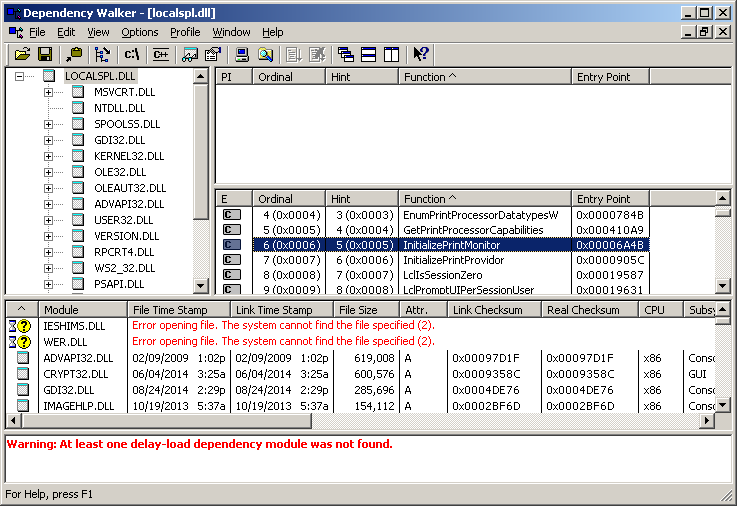
\includegraphics{images/depends.png}
	\caption{The Dependency Walker tool used to analyze the \emph{localspl.dll} of Windows Server 2003}
	\label{fig:DependencyWalker}
\end{figure}


\subsection{GNU strings}
The GNU strings utility reads any binary file and outputs all found sequences of printable characters.
It supports interpretation of the characters as ANSI and Unicode strings, which is a requirement for analyzing Windows applications that often use both character sets.
The tool reveals many interesting strings contained in Windows modules, for example:

\begin{itemize}
	\item Registry keys used to store the module's settings
	\item Paths to other related files
	\item Template data used by the module to fulfill its tasks
	\item Error messages (useful to get an idea what tasks are fulfilled by the module)
\end{itemize}

GNU strings is part of the Open-Source GNU Binutils package and shipped with many Linux distributions \cite{fsf2015strings}.
A Windows version of the tool is part of the \href{https://www.reactos.org/wiki/Build_Environment}{ReactOS Build Environment}.


\subsection{Rohitab Batra's API Monitor}
The \gls{API} Monitor by Rohitab Batra is a freely downloadable tool from \href{http://rohitab.com}{rohitab.com}.
It offers an efficient graphical user interface for monitoring the \gls{API} function calls of selected applications.
For \gls{API} functions known to the tool, the supplied parameter values are extracted and passed structures are decomposed.
The application can be enhanced to monitor additional \gls{API} functions by writing simple function definition files in \gls{XML}.
A screenshot of the tool is given in Figure~\ref{fig:APIMonitor}.
This one reveals that Windows' Spooler Server actually calls the Spooler Router function \texttt{AddJobW} when it receives a \texttt{StartDocPrinter} call over \gls{RPC}, despite the existence of a matching \texttt{StartDocPrinterW} function in the Spooler Router.
Passed parameters before and after the call are extracted and subsequent \gls{API} calls recorded.

\begin{figure}[h]
	\centering
	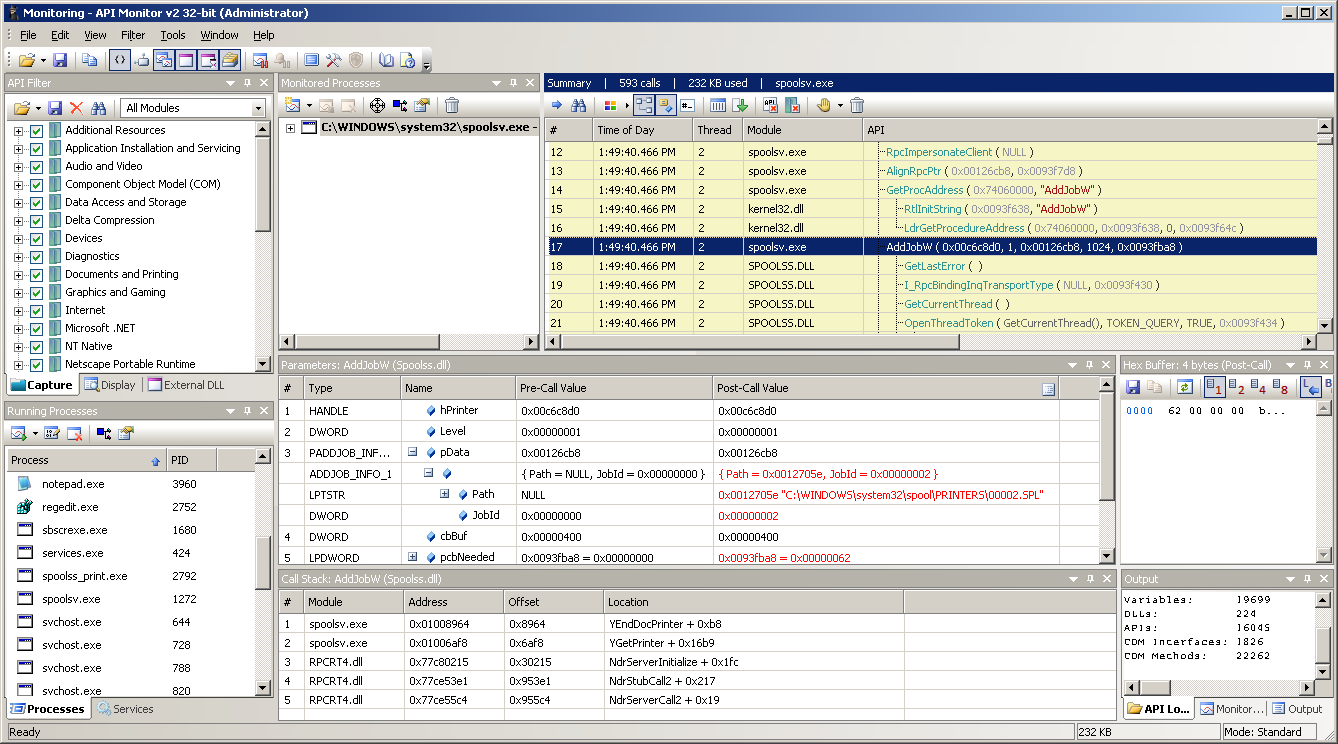
\includegraphics{images/apimon.png}
	\caption{Rohitab Batra's \glsdisp{API}{API} Monitor used to analyze an \glsdisp{RPC}{RPC} call to the Spooler Server in Windows Server 2003}
	\label{fig:APIMonitor}
\end{figure}


\subsection{WinDbg}
WinDbg is a debugger offered as a free download by Microsoft.
It supports debugging User-Mode and Kernel-Mode applications and is generally the debugger of choice for Windows driver developers due to its tight integration into the Microsoft development environment.
Kernel-Mode debugging can happen on the local system or on a remote computer that is connected through a Serial, FireWire, \gls{USB} or Ethernet cable.
In a next step, Windows is booted with the \gls{KD} Protocol enabled to let the debugger connect and afterwards break into every component of the operating system at any time.
This Protocol has also been adopted by the ReactOS Operating System to provide a debugging experience comparable to Windows.
That means, the same WinDbg application can be used to debug ReactOS just like a usual Windows environment.

WinDbg can retrieve information from \gls{PDB} files to provide single stepping through C/C++ source code files and detailed symbol information.
\gls{PDB} files are either generated by the Visual C++ compiler (for self-written applications) or downloaded from the Microsoft Symbol Server (for closed-source Windows components).
While latter ones do not reveal any source code of Windows components, the closed-source \gls{PDB} files make WinDbg aware of some variables and function names.
On top of this, WinDbg comes with a handful of extensions that provide several abstract views on the operating system state.
For example, this encompasses loaded processes and threads, bluescreen analysis, and hardware status information.
A typical WinDbg screen is shown in Figure~\ref{fig:WinDbg}.
With all these possibilities combined, WinDbg provides quite a powerful tool to gather information about any software under Windows or single step through it.


\begin{landscape}
	\begin{figure}
		\centering
		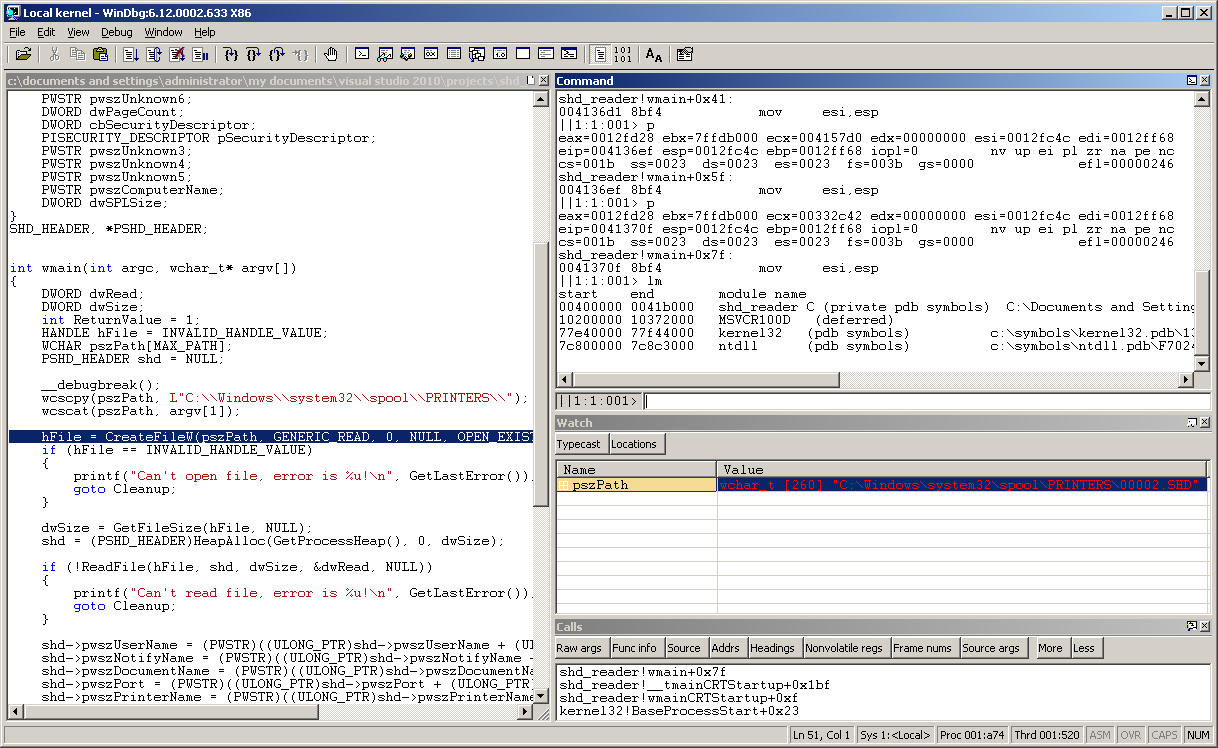
\includegraphics{images/windbg.png}
		\caption{WinDbg debugging a User-Mode application with loaded \glsdisp{PDB}{PDB} information in Windows Server 2003}
		\label{fig:WinDbg}
	\end{figure}
\end{landscape}

\chapter{Implementation}
\label{chp:implementation}
This chapter details the conducted research of the required components for the Printing Stack as well as their actual implementation.
The developed components build up the foundations for a ReactOS Printing Stack that maintains compatibility with Windows \gls{API} functions.


\section{Examination Of Available Code}
As a first step, the ReactOS codebase was examined to to figure out available and unavailable components as well as the quality of their code.
Prior to this work, the project's source tree merely provided a basic skeleton for a Spooler Server along with some Printing components imported from the WINE Project.
An inquiry to the original developer revealed that the Spooler Server skeleton was only added to let applications check the existence of that particular service.
The service did not serve any meaningful purpose, so it could be safely removed and implemented from scratch during the thesis work.

A further inspection of WINE's Printing components led to the conclusion that their code could not be reused either.
WINE only provides a compatible replacement of \emph{winspool.drv} to account for many standard cases of Printing applications.
But instead of forwarding calls to the remaining components of the Windows Printing Stack, WINE's \emph{winspool.drv} translates incoming Print Requests to \gls{CUPS} commands.
WINE's Spooler Server is only a basic service skeleton as well and additional \gls{DLL} files like \emph{spoolss.dll} and \emph{localspl.dll} are unimplemented in essential parts.
Due to these reasons, the WINE Printing components were removed from the tree as well.

On the plus side, the ReactOS ecosystem has matured enough to provide a working \gls{RPC} Server, compatible kernel functions and a Parallel Port Driver.
This allowed a clear focus on printing-related components during the thesis work.

The only other notable Open-Source project sharing similar goals is the Samba Project, which implements several components to let UNIX computers interact in a network with Windows machines.
These components also include support for Network Printing.
But due to Samba's focus on UNIX systems, only some interface information could be used.
No related code for the implementation of a ReactOS Printing Stack has been offered by the project.

After the ReactOS codebase had been completely examined, development on the new Printing Stack components could start.


\section{Defining The Interfaces}
Implementation on a ReactOS component providing compatibility with a Windows one begins by defining its \gls{API} functions in a so called \emph{SPEC} file.
The SPEC file format was invented to account for the differences in linker information file formats between the GNU Linker and the Microsoft Linker.
Additionally, one can denote a function as a \emph{stub} in a SPEC file and that function will be exported with a simple entry point.
If an application calls such a stub function, the call is reported through a text message, but nothing else happens.
This still allows other features of the application to work properly.
Without stub functions, the application may crash or not even load at all.
SPEC files are processed by the \emph{spec2def} utility during the ReactOS build process, which converts the information into a linker information file suitable for the used linker and generates the entry points for the stub functions.

The names of all provided \gls{API} functions in \emph{winspool.drv} and \emph{spoolss.dll} could easily be determined by opening the matching \gls{DLL} files from Windows Server 2003 in Dependency Walker and inspecting the Exports section.
Consequently, parameters for several basic Printing \glspl{API} were looked up on the web.
As these functions are fundamental to any application making use of Printing, the \href{http://msdn.microsoft.com}{MSDN Website} offers a detailed documentation on them.
After linking the documentation from both sources together, the SPEC files for \emph{winspool.drv} and \emph{spoolss.dll} were written.
Fundamental functions were added in all details while most of the other \glspl{API} were defined as stubs to allow a later implementation when necessary.

The Spooler Server process required a radically different approach to gain compatibility.
Its interfaces are not based on regular function calls, but use \gls{RPC} calls defined in \gls{IDL} files.
These cannot simply be revealed by a tool like Dependency Walker.
Instead, they usually require monitoring of the \gls{RPC} functions and reconstruction of the names and parameters.

The Samba Project has done this work for its Network Printing support and provides a corresponding \href{https://git.samba.org/?p=samba.git;a=blob;f=librpc/idl/spoolss.idl;hb=618af83d1bd07b12a9acc88b0d2111cab7a8bb2b}{\gls{IDL} file}.
A similar research has also been independently conducted in \cite{marchand2006netsvcs}.
Furthermore, Microsoft has begun to document the Print System \gls{RPC} Interface in 2007 and now provides a freely usable \gls{IDL} file covering a subset of the \gls{RPC} functions \cite{microsoft2014msrprn}.
By combining the information from these three sources, a detailed \gls{IDL} file could be constructed for defining the ReactOS Spooler Server interfaces.


\section{Choosing A Programming Language}
ReactOS components are either written in C or C++, with some performance-critical or processor-specific code written in Assembly language.
Due to the portability issues involved, Assembly language is only used as a last resort though.
It definitely offers no advantages for the development of a Printing Stack.

The remaining decision between C and C++ has been made based on compatibility requirements.
Advantages of C++ for a Printing Stack would lie in the object-oriented approach towards lists and strings.
The \gls{STL} shipped with every C++ development environment provides container classes like \texttt{list} and \texttt{vector} as well as \texttt{string} for handling character sequences of arbitrary length.
However, Windows exposes a pure C interface for its fundamental Printing Stack functions due to historical reasons.
Using C++ objects internally would require conversions between both data formats in every step.
This would basically lead to additional overhead and cancel out most advantages of C++ for the development of a Printing Stack.

Therefore, the choice fell on the C language for all developed components of the Printing Stack.
The unavailability of standard container classes in C is outweighed by the number of library functions ReactOS provides for development in C.


\section{Developing The Required Components}
As a first step towards an adequate ReactOS Printing Stack, a small test application called \emph{winspool\_print} was written in C.
It uses fundamental \gls{API} functions of the \emph{winspool.drv} component to send a file with arbitrary RAW data to a local Printer.
Afterwards, the goals of the development work were defined around this application:
The created ReactOS Printing Stack must implement all required \glspl{API} and components for getting \emph{winspool\_print} to work.
Code shall be written in a compatible and flexible way that easily allows a further addition of the not yet implemented features.

In particular, this led to the following components being developed:

\begin{itemize}
	\item \textbf{winspool.drv} \\
				The Spooler \gls{API} in \emph{winspool.drv} implements all character encoding dependent functions for the default single-byte character set and double-byte Unicode.
				For the beginning, only some Unicode functions have been implemented, because these are recommended for new applications.
				Future implemented single-byte character set functions will simply convert between both encodings and then call a corresponding Unicode function.
				Besides, more advanced Spooler \gls{API} functions not required for the \emph{winspool\_print} tool were added as simple stubs for now.
	
	\item \textbf{spoolsv.exe} \\
				The Spooler Server directly builds upon the \gls{IDL} file, which defines its complete \gls{RPC} communication interface.
				As a result, all 96 \gls{RPC} calls need to be implemented as functions inside \emph{spoolsv.exe}.
				Since many of them are unrelated to getting the basic \emph{winspool\_print} tool to work, some were just implemented to return the error code \texttt{ERROR\_INVALID\_FUNCTION} when being called.
				The others correctly perform Impersonation and pass the call to a Spooler Router function.
				
	\item \textbf{spoolss.dll} \\
				The Spooler Router has been implemented with the same subset of \gls{API} functions that were considered for \emph{winspool.drv}.
				Apart from this, the \gls{DLL} also provides fundamental Impersonation and Memory Management functions to all Printing components.
				Impersonation has been discussed in Section~\ref{sec:WindowsPrinting}.
				
				Due to the wide usage of these \glspl{API}, they received intensive \emph{Black-Box Testing}.
				That means, the functions were called with defined input data under Windows and their output was recorded.
				Based on the correlations between input and output, hypotheses were made and verified with further similar tests.
				Finally, enough information has been gathered to write compatible substitution code.
	
	\item \textbf{localspl.dll} \\
				For sending RAW data to a Printer, the Local Spooler in \emph{localspl.dll} needs to manage Printers, Print Jobs, Print Monitors and Print Processors as well as a list of Ports managed by Port Monitors.
				Support for Forms, Printer Drivers as well as their configuration data can be added at a later stage.
				
				In contrast to the Windows counterpart of \emph{localspl.dll}, the Port Monitor and Print Processor parts were sourced out into individual \gls{DLL} files for the ReactOS implementation.
				This decision logically separates such distinct components and follows the Windows Printing Architecture more closely.
				
	\item \textbf{winprint.dll} \\
				The variant of \emph{winprint.dll} implemented for ReactOS contains the default Print Processor called \emph{WinPrint}.
				Under Windows Server 2003, this one is part of \emph{localspl.dll} and supports \gls{EMF}, RAW and TEXT datatypes.
				To achieve the goal of getting \emph{winspool\_print} to work, code for processing the RAW datatype is needed.
				This code simply passes the data to the Port Monitor without altering it in any way.
				On the other hand, it has been developed flexible enough to account for a later addition of more datatypes.
				
	\item \textbf{localmon.dll} \\
				The Local Port Monitor is also part of \emph{localspl.dll} under Windows Server 2003, but has been sourced out into the \emph{localmon.dll} file for ReactOS.
				While the original Windows Local Port Monitor provides support for Parallel and Serial Ports along with Infrared Printers, support for the latter has not been implemented into the ReactOS counterpart yet.
				This decision originates from the unavailability of an Infrared Printer at the time of development as well as the added complexity that comes with a wireless link.
\end{itemize}

The implemented components are marked in yellow in Figures~\ref{fig:WindowsSpooling} and \ref{fig:WindowsPrinting}.
Making them usable for the intended purpose also required an integration into the ReactOS Build System.
This step is illustrated in the next section.


\section{Integrating The Components Into The ReactOS Build System}
The ReactOS Project features a Build System based on the \href{http://www.cmake.org/}{CMake} Build Automation Tool.
This system supports building ReactOS under Windows, Linux, or Mac OS X using either GCC or the Microsoft Visual C++ compiler.
In order to properly add the developed components to the operating system build process, several so-called \emph{CMakeLists} files have been written.
These are usual plain-text files editable with any text editor.
Each of them defines a module, its type (Application or \gls{DLL}), its target location in the operating system, the associated source code files, and the libraries it depends on.
This information is sufficient for CMake to call the corresponding compilers and linkers to build suitable binary files.


\section{Verification During Development}
One of the basic rules when writing operating system code is to make no assumptions at any stage \cite{ionescu2007reactos}.
The developed \glspl{API} will later be called by thousands of third-party applications.
This requires a developer to consider every possible case of calling a particular function and respond accordingly.

In the case of the Windows Printing Stack, a pure C \gls{API} is exposed.
It throws no exceptions and responds to failure cases by setting an appropriate return value and a Win32 Error Code \cite{msdn2015setlasterror}.
Such error codes can be very specific and some applications may implement code paths that check for a particular error code.
Therefore, developing a compatible reimplementation also requires figuring out the returned error code for each possible failure case.

The ReactOS Project is tackling this problem through \emph{Regression Tests}.
After verifying the behavior of an \gls{API} function under Windows, a developer usually writes a Regression Test that calls the function with defined input data and checks that it returns the verified output.
The test is then run under ReactOS to verify that the implementation of the function is compatible to the original.
In a next step, regularly running this test catches cases where changes in one module accidentally break functionality in another module.
Currently, the ReactOS Project runs all available Regression Tests after every commit to the source code repository.
The results are then parsed, inserted into a database and later searchable online through the \href{https://reactos.org/testman}{ReactOS Test Manager}.

Writing Regression Tests for \emph{winspool.drv} was straightforward due to the fact that this is a documented \gls{API} used in every Printing application.
For now, the test is only able to call deterministic informational functions though (like \texttt{GetPrint\-Processor\-Directory}).
Many other functions require the presence of a Printer, which is not guaranteed, and they also behave differently based on the type of Printer connected.
Consequently, these functions are not yet covered by the Regression Tests.

However, other components of the Printing Stack are harder to test.
A prominent example is \emph{localspl.dll}.
Under Windows, the Spooler Server, Spooler Router, and this \gls{DLL} are intertwined with each other in a way that prevents loading \emph{localspl.dll} in any other application.

Nevertheless, it was possible to verify the behavior of its Print Provider functions under Windows by using a different approach:
The code for testing the function was put into a self-written \gls{DLL} file.
A standalone application was then launched with highest privileges in order to let it use the Windows \texttt{CreateRemoteThread} \gls{API} function, which creates a new thread in the running Spooler Server process \cite{msdn2015createremotethread}.
The created thread loaded the testing code from the \gls{DLL} file and by running that code in a thread of the Spooler Server, it can access all functions of \emph{localspl.dll}.
Eventually, this testing method offered unique insights into the internal behavior of the Local Spooler.
These were used to develop a compatible replacement and verify it against the original.

However, gathering such information from existing components is only one part of developing a Printing Stack for ReactOS.
At a later development stage, the design of custom data structures also became necessary.
This step is further discussed in the next section.


\section{Designing The Data Structures}
One of the Local Spooler's primary tasks is managing a changing number of Printers, Print Monitors, and Print Processors in a list.
Along with every Printer comes a prioritized Job Queue.
The exposed Spooler \gls{API} allows to add, remove, and enumerate items from these lists.
Moreover, it also allows Print Jobs to be reprioritized or to get their Job index in the list.
Calling these \glspl{API} often causes lookup operations to be performed in the background.

Windows offers a variety of abstract data types ready to use in Kernel-Mode and User-Mode applications.
Two of them were further analyzed with a focus on usability for the Printing components:

\begin{itemize}
	\item \textbf{Doubly-linked Lists} \\
				A Doubly-linked List implemented through Windows' \texttt{LIST\_ENTRY} structure is the simplest abstract data type for these tasks.
				It can do standard operations like additions, enumerations, and removals always in $\mathcal{O}(1)$, provided that no lookup is necessary beforehand.
				Lookups are an expensive operation for Linked Lists though, because they are only doable in linear time.
				Consequently repriorizing a Job, which involves deleting and reinserting an element at another position, needs linear time as well and shares the same $\mathcal{O}(n)$ complexity.
				Therefore, the focus shifted to other abstract data types.
	
	\item \textbf{Generic Tables} \\
				The Windows Run-Time Library also offers a data structure called \emph{General Table}.
				Depending on the compile options, this one is either implemented as an \gls{AVL} tree or a Splay Tree \cite{osr2008splaytrees}.
				Both are comparable in complexity, so they will not be discussed separately.
				The tree structures also offer $\mathcal{O}(1)$ complexity for additions and removals on average.
				Lookups and consequently repriorizations are usually faster, with a complexity of $\mathcal{O}(\log n)$ on average.
				On the other hand, enumerations bear a higher complexity, since finding the next element of an in-order traversal is a non-trivial operation.
				
				For usage inside the Printing components, there is another major downside compared to the \texttt{LIST\_ENTRY}-based implementation of Doubly-linked Lists:
				Every insertion allocates a new block of memory instead of reusing the existing one.
				Among added overhead, this makes pointer references more complicated, because the element address is only known after the insertion.
				Another disadvantage is the opaque structure of Generic Tables, which allows no further extensions.
				Due to the already high complexity of enumerations, this makes figuring out the element index inside Generic Tables an even more expensive operation, with a complexity greater than $\mathcal{O}(n)$.
\end{itemize}

As both integrated abstract data types were not satisfying the requirements, a data structure adjusted to the needs of the Printing components has been developed.


\subsection{Skip Lists}
Skip Lists were introduced by William Pugh in 1990 as an easy to implement alternative to balanced trees \cite{pugh1990skiplists}.
They build upon the structure of singly-linked lists, but every node features an array of pointers instead of a single pointer to a next node.
The array size is predefined at compile time.

Every time a node is inserted into a Skip List, a geometrically distributed random function for $p = 0.5$ is called to return a \emph{level} for it.
The level determines how many pointers to a next node are used.
Consequently, it can be between 1 and the array size.
In the long run, every next higher level appears only half as often as a previous one due to the geometric distribution.
This results in a structure as exemplarily depicted in Figure~\ref{fig:SkipList}.

Just like for singly-linked lists, the first pointer always links to the directly adjacent element.
The second pointer connects all nodes that received a level of 2 or higher.
This goes on for the third pointer, the fourth pointer, etc.

Such a probabilistic approach generates a data structure with lookup properties comparable to binary trees.
It only involves a cheap random function to achieve this instead of enforcing complex and expensive rebalancing operations.

Lookups are implemented by starting from the head node and checking the next node on the highest used level.
The code then passes all nodes on this level coming before the node it is looking for.
When a final node on one level is reached, the code goes down a level and continues there.
These steps are repeated until the first level and the desired node is reached.
The advantageous distribution of levels across the Skip List leads to an average complexity of $\mathcal{O}(\log n)$ for lookups.

Insertions and removals in Skip Lists always need to perform a lookup first.
However, the remaining operations are doable in $\mathcal{O}(1)$, so the final complexity for both operations is $\mathcal{O}(\log n)$ too.

\begin{figure}[t]
	\centering
	
	\begin{tikzpicture}
		\node[cf_skiplistitem=5] (H) {L4 \nodepart{two} L3 \nodepart{three} L2 \nodepart{four} L1 \nodepart{five} Head};
		\node[cf_skiplistitem=2, right = of H.south, anchor = south] (5) {\nodepart{two} 5};
		\node[cf_skiplistitem=3, right = of 5.south, anchor = south] (7) {\nodepart{three} 7};
		\node[cf_skiplistitem=5, right = of 7.south, anchor = south] (10) {\nodepart{five} 10};
		\node[cf_skiplistitem=4, right = of 10.south, anchor = south] (15) {\nodepart{four} 15};
		\node[cf_skiplistitem=2, right = of 15.south, anchor = south] (16) {\nodepart{two} 16};
		\node[cf_skiplistitem=2, right = of 16.south, anchor = south] (19) {\nodepart{two} 19};
		\node[cf_skiplistitem=3, right = of 19.south, anchor = south] (23) {\nodepart{three} 23};
		
		\path [cf_line] (H.one east) -- (10.one west |- H.one east);
		\path [cf_line] (H.two east) -- (10.two west |- H.two east);
		\path [cf_line] (H.three east) -- (7.one west |- H.three east);
		\path [cf_line] (H.four east) -- (5.one west |- H.four east);
		\path [cf_line] (5.one east) -- (7.two west |- 5.one east);
		\path [cf_line] (7.one east) -- (10.three west |- 7.one east);
		\path [cf_line] (7.two east) -- (10.four west |- 7.two east);
		\path [cf_line] (10.two east) -- (15.one west |- 10.two east);
		\path [cf_line] (10.three east) -- (15.two west |- 10.three east);
		\path [cf_line] (10.four east) -- (15.three west |- 10.four east);
		\path [cf_line] (15.two east) -- (23.one west |- 15.two east);
		\path [cf_line] (15.three east) -- (16.one west |- 15.three east);
		\path [cf_line] (16.one east) -- (19.one west |- 16.one east);
		\path [cf_line] (19.one east) -- (23.two west |- 19.one east);
	\end{tikzpicture}
	
	\caption{Example of a Skip List with four pointers for each node}
	\label{fig:SkipList}
\end{figure}

For ReactOS Printing components, the Skip List has been implemented in a way that it does not copy the element data.
Instead, it only saves a pointer to the data inside a node.
This prevents overhead and keeps previous pointer references to the element intact.

The simple structure of Skip Lists also allows for three extensions not found in known implementations:

\begin{itemize}
	\item \textbf{Reduction of comparisons} \\
				A lookup operation in any data structure requires multiple comparisons to be performed.
				To allow for every possible sorting order, the comparison is usually implemented by calling a previously specified Compare routine.
				As calling a function can be an expensive operation, an extension was proposed in 1990 to reduce the number of required comparisons.
				This is done by remembering the last compared element and never comparing the same element twice during the lookup \cite{pugh1990cookbook}.
				The extension has been implemented into the Skip List for the Printing components.

	\item \textbf{Fast lookup of element indexes} \\
				A concept for looking up an element by index in a Skip List has also been proposed in \cite{pugh1990cookbook}.
				It works by introducing an array, which keeps information about the distance to each other node.
				An exemplary Skip List with distance information is depicted in Figure~\ref{fig:SkipListWithDistance}.
				
				Maintaining these distance arrays requires slightly more algorithm complexity in the insertion and deletion functions.
				On the plus side, lookups can now return the element index as well while still keeping the same $\mathcal{O}(\log n)$ complexity on average.
				Such a lookup algorithm is given in Algorithm~\ref{alg:LookupElementSkiplist}.
				
	\item \textbf{Insertion of elements at the end of the list} \\
				A common task in Printing is adding a new Print Job with default priority.
				Such jobs are always inserted at the end of the Job List.
				Nevertheless, the standard insertion function would perform multiple expensive calls to the Compare routine to reach the Skip List tail.
				
				Therefore, an optimized function called \texttt{InsertTailElementSkiplist} has been introduced for the ReactOS Skip List implementation.
				This function simply takes the shortest route to reach the end of the Skip List without the overhead of calling the Compare routine.
\end{itemize}

\begin{figure}[t]
	\centering
	
	\begin{tikzpicture}
		\node[cf_skiplistitem=5] (H) {L4 \nodepart{two} L3 \nodepart{three} L2 \nodepart{four} L1 \nodepart{five} Head};
		\node[cf_skiplistitem=2, right = of H.south, anchor = south] (5) {\nodepart{two} 5};
		\node[cf_skiplistitem=3, right = of 5.south, anchor = south] (7) {\nodepart{three} 7};
		\node[cf_skiplistitem=5, right = of 7.south, anchor = south] (10) {\nodepart{five} 10};
		\node[cf_skiplistitem=4, right = of 10.south, anchor = south] (15) {\nodepart{four} 15};
		\node[cf_skiplistitem=2, right = of 15.south, anchor = south] (16) {\nodepart{two} 16};
		\node[cf_skiplistitem=2, right = of 16.south, anchor = south] (19) {\nodepart{two} 19};
		\node[cf_skiplistitem=3, right = of 19.south, anchor = south] (23) {\nodepart{three} 23};
		
		\path [cf_line] (H.one east) -- (10.one west |- H.one east);
		\path [cf_line] (H.two east) -- (10.two west |- H.two east);
		\path [cf_line] (H.three east) -- (7.one west |- H.three east);
		\path [cf_line] (H.four east) -- (5.one west |- H.four east);
		\path [cf_line] (5.one east) -- (7.two west |- 5.one east);
		\path [cf_line] (7.one east) -- (10.three west |- 7.one east);
		\path [cf_line] (7.two east) -- (10.four west |- 7.two east);
		\path [cf_line] (10.two east) -- (15.one west |- 10.two east);
		\path [cf_line] (10.three east) -- (15.two west |- 10.three east);
		\path [cf_line] (10.four east) -- (15.three west |- 10.four east);
		\path [cf_line] (15.two east) -- (23.one west |- 15.two east);
		\path [cf_line] (15.three east) -- (16.one west |- 15.three east);
		\path [cf_line] (16.one east) -- (19.one west |- 16.one east);
		\path [cf_line] (19.one east) -- (23.two west |- 19.one east);
		
		\path [cf_label] (H.one east) edge node [above] {3} (10.one west |- H.one east);
		\path [cf_label] (H.two east) edge node [above] {3} (10.two west |- H.two east);
		\path [cf_label] (H.three east) edge node [above] {2} (7.one west |- H.three east);
		\path [cf_label] (H.four east) edge node [above] {1} (5.one west |- H.four east);
		\path [cf_label] (5.one east) edge node [above] {1} (7.two west |- 5.one east);
		\path [cf_label] (7.one east) edge node [above] {1} (10.three west |- 7.one east);
		\path [cf_label] (7.two east) edge node [above] {1} (10.four west |- 7.two east);
		\path [cf_label] (10.two east) edge node [above] {1} (15.one west |- 10.two east);
		\path [cf_label] (10.three east) edge node [above] {1} (15.two west |- 10.three east);
		\path [cf_label] (10.four east) edge node [above] {1} (15.three west |- 10.four east);
		\path [cf_label] (15.two east) edge node [above] {3} (23.one west |- 15.two east);
		\path [cf_label] (15.three east) edge node [above] {1} (16.one west |- 15.three east);
		\path [cf_label] (16.one east) edge node [above] {1} (19.one west |- 16.one east);
		\path [cf_label] (19.one east) edge node [above] {1} (23.two west |- 19.one east);
	\end{tikzpicture}
	
	\caption{Example of a Skip List maintaining distance information between nodes}
	\label{fig:SkipListWithDistance}
\end{figure}

With these extensions, the Skip List performs very well for common tasks of the Printing Stack.
The average complexity of every single Skip List operation never exceeds $\mathcal{O}(\log n)$.
For ReactOS, a Skip List has been implemented with 16 pointers per element for managing Printers and Print Jobs.
This number of pointers keeps the average algorithm performance for up to $2^{16} = 65536$ elements.
A small test suite has been added to guarantee stability and reliability of the abstract data type implementation.


\subsection{Fast Random Number Generator}
\label{sec:FastRNG}
As noted beforehand, the implementation of a Skip List depends on a Generator returning geometrically distributed random numbers for $p = 0.5$.
In fact, the Generator needs to output an integer between 1 and the array size.
It does not need to produce cryptographically secure random numbers though.
Even more, the numbers may be fully predictable, because only their distribution is relevant for the Skip List concept to work.

With these given requirements, it was decided to integrate a custom Random Number Generator into the Skip List code instead of depending on an operating system function.
Designing a custom Random Number Generator would go far beyond the scope of this thesis.
To make a simple Generator available for nonspecialists, Stephen Park and Keith Miller proposed a variant of the \gls{LCG} in 1988, which is now known as the \emph{Minimal Standard Random Number Generator} \cite{parkmiller1988rng}.

The Skip List's \texttt{\_GetRandomLevel} function makes use of this Random Number Generator using the revised parameters $a = 48271$ and $n = 2147483647$ \cite{parkmillerstockmeyer1993rng}.
As the returned numbers may be completely predictable, a fixed seed of 1 was defined in the code.

In the beginning, it outputs 31 uniformly distributed random bits.
A bitshift to the right is then performed to shift out some bits and only leave one bit for every possible level (as configured through the array size).
This method limits the possible Skip List node array size to 31 pointers.
Anyway, such a size would be enough to account for up to $2^{31}$ elements while still having a data structure that keeps the average algorithm complexity.
For the Printing Stack, a Skip List with 16 possible levels is used, so half of the random bits are shifted out.

Finally, the uniform distribution is turned into a geometric distribution for $p = 0.5$ by using the \emph{Bit Scan Forward} processor instruction.
This instruction counts the bits set to one from the least-significant bit to the most-significant bit and returns the position of the first zero.
Hence, a zero in the first bit has a probability of $0.5^1 = 0.5$, a zero in the first two bits has a probability of $0.5^2 = 0.25$, a zero in the first three bits has a probability of $0.5^3 = 0.125$, and so on.
As a result, this method delivers a geometric distribution for $p = 0.5$ efficiently.

The full \texttt{\_GetRandomLevel} listing can be found in Appendix~\ref{sec:GetRandomLevel}.
The function is simple enough to be declared as an inline function.


\begin{algorithm}[t]
	\caption{Looking up an element and its 1-based index in a Skip List}
	\label{alg:LookupElementSkiplist}
	\begin{algorithmic}[1]
		\Procedure{LookupElementSkiplist}{$Skiplist$, $Element$}
			\State $Index \gets 1$
			\State $Node \gets Skiplist.Head$
			\newline
			\For{$i = Skiplist.MaximumLevel \to 1$}
				\While{$Node.Next[i].Element < Element$}
					\State $Index \gets Index + Node.Distance[i]$
					\State $Node \gets Node.Next[i]$
				\EndWhile
			\EndFor
			\newline
			\State $Node \gets Node.Next[0]$
			\If{$Node.Element \neq Element$}
				\State \textbf{return} $\varnothing$
			\EndIf
			\newline
			\State \textbf{return} $(Node.Element, Index)$
		\EndProcedure
	\end{algorithmic}
\end{algorithm}

\chapter{Evaluation}
In this chapter, the developed components are evaluated through specific individual tests.
These tests do not only cover the actual components making up the Printing Stack, but also verify the correctness of the Skip List implementation.


\section{Verifying The Random Number Generator}
In Section~\ref{sec:FastRNG}, a fast Random Number Generator has been developed that is designed to return geometrically distributed numbers denoting Skip List levels.
The probability parameter of this Generator is defined as $p = 0.5$.
Achieving a sufficiently geometric distribution of Skip List levels is crucial for the Skip List performance.
The average complexity of the algorithms involved cannot be reached if the Skip List levels follow a different distribution.

To verify the distribution of levels returned by the Random Number Generator, a test application has been written.
It calls the Random Number Generator a predefined number of times to simulate the distribution of levels for a Skip List with the same element count.
Logarithmic plots of the results of simulations with 1000 and 65536 elements are provided in Figure~\ref{fig:ElementDistribution}.

In both cases, the results show an approximate geometric distribution for the lower levels with some outliers for higher levels.
As the number of elements is significantly lower on higher levels, these outliers are negligible.
Generally spoken, the more elements are added to a Skip List, the more their assigned levels converge to a geometric distribution.
In total, this test shows that the implemented Random Number Generator is feasible to get the desired distribution for the Skip List algorithms.

\begin{figure}[t]
	\centering
	
	\begin{tikzpicture}
		\begin{axis}[
			scale=0.75,
			title={1000 Elements},
			xlabel={Level},
			xmax=16,
			ymin=0.5,
			ylabel={Element Count},
			ymode=log,
			log basis y=2,
			ytick={1,8,64,512}
		]
			\addplot table {plots/16_levels_1000_elements.csv};
		\end{axis}
	\end{tikzpicture}
	\hspace{8mm}
	\begin{tikzpicture}
		\begin{axis}[
			scale=0.75,
			title={65536 Elements},
			xlabel={Level},
			xmax=16,
			ymin=0.5,
			ymode=log,
			log basis y=2,
			ytick={1,32,1024,32768}
		]
			\addplot table {plots/16_levels_65536_elements.csv};
		\end{axis}
	\end{tikzpicture}
	
	\caption{Distribution of 1000 and 65536 elements across the levels of a 16-level Skip List using the Minimal Standard Random Number Generator}
	\label{fig:ElementDistribution}
\end{figure}


\section{Testing The Skip List Implementation}
As the Skip List is an integral component of the developed Printing Stack, its algorithms received additional unit testing.
In particular, the Skip List for the Printing Stack includes distance arrays for each element to allow a fast lookup of element indexes.
This requires the insertion and deletion functions to update both pointers and distances with every operation.

To test all implemented Skip List functions, another test program has been written.
It utilizes a Skip List that manages plain integer numbers and sorts them in ascending order.
The test first adds 40 random numbers to the list.
In a next step, all numbers in the range 0 to 29 are deleted again.
Finally, another batch of 40 random numbers is added to the Skip List.
Two lookup operations are performed afterwards, one by index and one by looking for a specific integer.
In the end, the structure of the final Skip List is drawn on the screen.
The drawing process makes use of both the pointer and distance information.
An exemplary output of the test program is depicted in Figure~\ref{fig:skiplist_test}.

By calling these individual functions in this specific order, all aspects of the Skip List are tested.
Typical bugs in abstract data type implementations can be caught, like corrupted structures after an operation, off-by-one mistakes in loops, or similar.
The final dump of the resulting structure allows a visual check of the entire Skip List.
In case of a bad link to a next element or a wrongly calculated distance, an element would appear misaligned.

\begin{figure}[b]
	\centering
	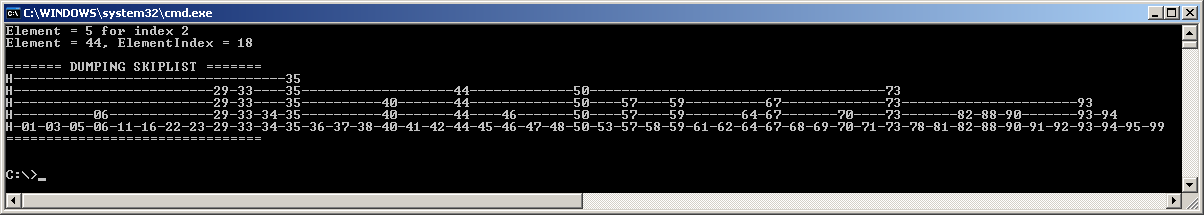
\includegraphics{images/skiplist_test.png}
	\caption{Exemplary output of the Skip List test program}
	\label{fig:skiplist_test}
\end{figure}


\section{Testing The ReactOS Printing Stack In A Virtual Machine}
After individual tests of crucial components, the developed Printing Stack as a whole needed to be tested.
This has been accomplished by building an ISO~9660 image file for the entire ReactOS Operating System, including the newly developed Printing Stack components and the \emph{winspool\_print} test program.
The ReactOS Build System provides the target \emph{bootcd} for this purpose.
Calling this CMake target builds all operating system components and finally creates an ISO~9660 image file.
Instead of using the default GCC compiler, the operating system has been built using Microsoft Visual C++.
This creates the necessary \gls{PDB} files to enable source-level debugging with WinDbg.

As neither Printer Drivers nor Printer Setup functions exist at this stage of the Printing Stack, Printers cannot be installed through the operating system yet.
Without an installed Printer, the Printing Stack cannot be tested though.
To circumvent this problem, the ReactOS installation data has been modified to always set up a dummy Printer connected to the first Parallel Port.
Without a corresponding Printer Driver, this dummy Printer is still able to forward RAW data to the connected real Printer.
As no other datatype nor datatype conversions are supported by now, such a dummy Printer is sufficient for all testing scenarios.

To catch outstanding code bugs early, it has been decided to use a Virtual Machine for testing.
This allows to develop and test on the same computer as well as mounting the created ISO~9660 image file in a virtual CD drive instead of burning it to a blank CD.
While many different Virtualization products exist today, only some were suitable for evaluating the Printing Stack.
This is due to the fact that the Printing Stack outputs data over a Parallel Port.
For this purpose, the free \href{http://www.vmware.com/products/player}{VMware Player} software turned out to be a viable solution, because it offers a virtual Parallel Port, whose output can be redirected into a file.
The returned data can then be examined to validate the correctness of the Printing Stack.

VMware Player has also been configured to emulate a virtual Serial Port and redirect this one to a bidirectional pipe.
The WinDbg debugger can then connect to this pipe and act like it was debugging ReactOS on a computer connected through a physical Serial Cable.

By the use of VMware and WinDbg, several bugs have been caught and fixed in a relatively short time.
Using a Virtual Machine instead of Real Hardware for these tests has also simplified the deployment of fixes:
System components could be exchanged by turning off the Virtual Machine, mounting its virtual Hard Disk on the Host Computer and rebooting ReactOS.

At the end of the testing and fixing phase, the Printing components have finally become robust enough for the \emph{winspool\_print} tool.
The set of implemented \gls{API} calls can be used reliably to send RAW Printing data to the Parallel Port.
Examination of the redirected Parallel Port output has revealed that a Printer would receive properly formatted data.


\section{Running The ReactOS Printing Stack On Real Hardware}
The final evaluation of the developed Printing Stack happened on a real computer connected to a physical Printer.
For this test, a Lenovo ThinkPad X61 with Docking Station has been chosen.
This machine's hardware components are known to be supported by ReactOS out of the box without relying on third-party hardware drivers.
The Docking Station offers Parallel and Serial Ports not provided by the laptop itself.

Preferably, a Dot-Matrix Printer would have been connected to the Parallel Port of this laptop.
Such Printers work character-wise, meaning that they do not await a full page in a Control Language, but output every transmitted character as soon as it arrives.
Due to the unavailability of a Dot-Matrix Printer at the time of testing, a Hewlett-Packard DeskJet 710C Inkjet Printer has been chosen instead.
This particular Printer expects all incoming data in Hewlett-Packard's proprietary \gls{PPA} Control Language.
The \gls{PPA} Language is implemented into the included Windows Device Driver, but otherwise largely undocumented.
However, Windows Printer Drivers are not usable in ReactOS before the \gls{GDI} part of the Printing Stack has been implemented.
Therefore, another solution was necessary to prepare data in \gls{PPA} Language.

This solution has been found in the \emph{PNM2PPA} tool.
PNM2PPA is a program that converts an input image in Portable Pixmap raster format into appropriate \gls{PPA} data for supported Hewlett-Packard Printers \cite{pnm2ppa2015}.
It is usually used in conjunction with the GhostScript software, which converts documents in PostScript language into raster formats.
Together both applications build a filter chain for \gls{CUPS} users to let them print on \gls{PPA} Printers.

As a result of this, a single page document was prepared on a different computer.
This document was first converted into PostScript, then processed into a raster image using GhostScript until PNM2PPA finally produced data in \gls{PPA} format.
The created \gls{PPA} file was then transferred to the laptop running ReactOS.
Finally, the \emph{winspool\_print} tool read the \gls{PPA} file and transmitted correctly formatted data to the DeskJet Printer using \gls{API} functions of the Printing Stack.
The Printer reacted accordingly and printed out the previuosly prepared document.

This final step of testing has shown that the implemented features of the Printing Stack can properly communicate with Printers.

\chapter{Conclusion}
This thesis presents a Printing Stack for the ReactOS Operating System, which offers compatibility with Windows Printing \gls{API} functions and extensibility for future additions.

Through extensive research in advance, the official Microsoft documentation for the Windows Printing Stack has been complemented by additional information.
An overview of the components involved and their mutual dependencies has been given.

Based on the gathered information, a compatible replacement has been developed for each fundamental component.
By the consequent usage of various verification methods during the development process, reliable code and compatibility to Windows Server 2003 is guaranteed.
Implementing communication between applications and the Printing Stack consistently over \gls{RPC} paves the way for a future integration of ReactOS-based Print Servers into a networked environment.

The Skip List abstract data type has been introduced to address the need for a flexible list structure inside Printing Stack components.
Its implemented extensions provide performance enhancements when handling large sets of elements.

Final testing of the Printing Stack inside a Virtual Machine and on Real Hardware has demonstrated the functioning of the developed framework.

\bigskip

Within the scope of this bachelor's thesis, only the foundations of the Printing Stack could be implemented.
The next logical task would be adding support for native Windows Printer Drivers, which convert \gls{EMF} data into Printer Control Language.
Along with this task comes the implementation of fundamental \gls{GDI} functions for Printing, e.g. \texttt{StartDoc} and \texttt{EndDoc}.

In order to provide an intuitive and satisfying user experience, the ReactOS Printing Stack also requires several user interface components to be developed, which guide the user through the installation, configuration, and management of available Printers.

Finally, a modern operating system needs to provide support for a wide variety of Printers out of the box.
Due to the vast number of different Printers available, the development focus should lie on Generic Drivers implementing common Printer Control Languages.
One example of this is Adobe PostScript.

\bigskip

To put it in a nutshell, Printing is an integral feature of modern desktop operating systems.
Providing a suitable Printing Stack for the ReactOS Project enriches the user experience and improves compatibility with many popular applications.
All in all, this step makes more usage scenarios imaginable for the Open-Source Windows-compatible operating system.

 						% this file contains includes for the individual chapters

\appendix 								% uncomment these two lines if you wish
\appendixintro
\chapter{Listings}
This appendix provides the actual C code for some implemented functions discussed in Chapter~\ref{chp:implementation}.


\section{\_GetRandomLevel function}
\label{sec:GetRandomLevel}
The \texttt{\_GetRandomLevel} function has been introduced in Section~\ref{sec:FastRNG}.
It implements the Random Number Generator required for determining the level of a new element added to a Skip List.
\bigskip

\begin{lstlisting}
// Define SKIPLIST_LEVELS to the maximum number of levels the Skip List shall have.
#define SKIPLIST_LEVELS    16

C_ASSERT(SKIPLIST_LEVELS >= 1);
C_ASSERT(SKIPLIST_LEVELS <= 31);

static __inline CHAR
_GetRandomLevel()
{
    // Using a simple fixed seed and the Park-Miller Lehmer Minimal Standard Random Number Generator gives an acceptable distribution for our "random" levels.
    static DWORD dwRandom = 1;

    DWORD dwLevel = 0;
    DWORD dwShifted;

    // Generate 31 uniformly distributed pseudo-random bits using the Park-Miller Lehmer Minimal Standard Random Number Generator.
    dwRandom = (DWORD)(((ULONGLONG)dwRandom * 48271UL) % 2147483647UL);

    // Shift out (31 - SKIPLIST_LEVELS) bits to the right to have no more than SKIPLIST_LEVELS bits set.
    dwShifted = dwRandom >> (31 - SKIPLIST_LEVELS);

    // BitScanForward doesn't operate on a zero input value.
    if (dwShifted)
    {
        // BitScanForward sets dwLevel to the zero-based position of the first set bit (from LSB to MSB).
        // This makes dwLevel a geometrically distributed value between 0 and SKIPLIST_LEVELS - 1 for p = 0.5.
        BitScanForward(&dwLevel, dwShifted);
    }

    // dwLevel can't have a value higher than 30 this way, so a CHAR is more than enough.
    return (CHAR)dwLevel;
}
\end{lstlisting}


\section{\_RpcWritePrinter implementation}
\label{sec:RpcWritePrinter}
\texttt{\_RpcWritePrinter} is one of the \gls{RPC} server functions implemented in the Spooler Server.
It serves as an example how most of the \gls{RPC} calls are implemented.
Basically, Impersonation is performed, the corresponding Spooler Router function called, and finally the security context reverted back to the system context.
This process is further illustrated in Figure~\ref{fig:WritePrinterProcessing}.
\bigskip

\begin{lstlisting}
DWORD
_RpcWritePrinter(WINSPOOL_PRINTER_HANDLE hPrinter, BYTE* pBuf, DWORD cbBuf, DWORD* pcWritten)
{
    DWORD dwErrorCode;

    dwErrorCode = RpcImpersonateClient(NULL);
    if (dwErrorCode != ERROR_SUCCESS)
    {
        ERR("RpcImpersonateClient failed with error %lu!\n", dwErrorCode);
        return dwErrorCode;
    }

    WritePrinter(hPrinter, pBuf, cbBuf, pcWritten);
    dwErrorCode = GetLastError();

    RpcRevertToSelf();
    return dwErrorCode;
}
\end{lstlisting}

 						% to add an appendix

 					

\end{document}
